\documentclass{beamer}
\usepackage[utf8]{inputenc}

\usetheme{Madrid}
\usecolortheme{default}
\usepackage{amsmath}
\usepackage{amssymb,amsfonts,amsthm}
\usepackage{txfonts}
\usepackage{tkz-euclide}
\usepackage{listings}
\usepackage{adjustbox}
\usepackage{array}
\usepackage{tabularx}
\usepackage{gvv}
\usepackage{lmodern}
\usepackage{circuitikz}
\usepackage{tikz}
\usepackage{graphicx}

\setbeamertemplate{page number in head/foot}[totalframenumber]

\usepackage{tcolorbox}
\tcbuselibrary{minted,breakable,xparse,skins}



\definecolor{bg}{gray}{0.95}
\DeclareTCBListing{mintedbox}{O{}m!O{}}{%
  breakable=true,
  listing engine=minted,
  listing only,
  minted language=#2,
  minted style=default,
  minted options={%
    linenos,
    gobble=0,
    breaklines=true,
    breakafter=,,
    fontsize=\small,
    numbersep=8pt,
    #1},
  boxsep=0pt,
  left skip=0pt,
  right skip=0pt,
  left=25pt,
  right=0pt,
  top=3pt,
  bottom=3pt,
  arc=5pt,
  leftrule=0pt,
  rightrule=0pt,
  bottomrule=2pt,
  toprule=2pt,
  colback=bg,
  colframe=orange!70,
  enhanced,
  overlay={%
    \begin{tcbclipinterior}
    \fill[orange!20!white] (frame.south west) rectangle ([xshift=20pt]frame.north west);
    \end{tcbclipinterior}},
  #3,
}
\lstset{
    language=C,
    basicstyle=\ttfamily\small,
    keywordstyle=\color{blue},
    stringstyle=\color{orange},
    commentstyle=\color{green!60!black},
    numbers=left,
    numberstyle=\tiny\color{gray},
    breaklines=true,
    showstringspaces=false,
}
\title{1.9.14}
\date{27th August, 2025}
\author{Vishwambhar - EE25BTECH11025}

\begin{document}

\frame{\titlepage}
\begin{frame}{Question}
If $\vec{P}=\brak{2,2}$, $\vec{Q}=\brak{-4,-4}$, and $\vec{R}=\brak{5,-8}$ are the vertices of a triangle $\Delta PQR$, then find the length of the median through $\vec{R}$.\\
\end{frame}

\begin{frame}{allowframebreaks}
\frametitle{Midpoint of $\vec{Q}-\vec{P}$}
Given position vectors of the points are:
\begin{align}
    \vec{P}=\myvec{2\\2},
    \vec{Q}=\myvec{-4\\-4},
    \vec{R}=\myvec{5\\-8}
\end{align}
Let the midpoint of vector $\vec{Q}-\vec{P}$ be $\vec{M}$:
\begin{align}
    \vec{M}=\frac{1}{2}\vec{P}+\frac{1}{2}\vec{Q}\\
    \vec{M}=\myvec{1\\1}+\myvec{-2\\-2}\\
    \vec{M}=\myvec{-1\\-1}
\end{align}
\end{frame}

\begin{frame}[fragile]
\frametitle{Length of Median}
\begin{align}
    \vec{M}-\vec{R}=\myvec{-1\\-1}-\myvec{5\\-8}\\
    \vec{M}-\vec{R}=\myvec{-6\\7}
\end{align}

The length of the median:
\begin{align}
    ||\vec{M}-\vec{R}||=\sqrt{\brak{-6}^2+\brak{7}^2}\\
    ||\vec{M}-\vec{R}||=\sqrt{85}\approx9.219
\end{align}

Thus the length of the median of the triangle through $\vec{R}$ is $\sqrt{85}\approx9.219$.
\end{frame}

\begin{frame}[fragile]
    \frametitle{C Code}
    \begin{lstlisting}
#include <stdio.h>

void get_points(double *points) {
    points[0] = 5;   points[1] = -8;   // R
    points[2] = -4;  points[3] = -4;   // Q
    points[4] = 2;   points[5] = 2;    // P
}
    \end{lstlisting}
\end{frame}

\begin{frame}[fragile]
    \frametitle{Python Code}
    \begin{lstlisting}
import sys
import math
import numpy as np
import matplotlib.pyplot as plt
import ctypes

problem = ctypes.CDLL('/home/ganachari-vishwmabhar/ee1030-2025/EE25BTECH11025/ASSIGNMENTS/matgeo/1.5.13/codes/problem.so')
    \end{lstlisting}
\end{frame}

\begin{frame}[fragile]
    \frametitle{Python Code}
    \begin{lstlisting}
P = np.array([2, 2])
Q = np.array([-4, -4])
R = np.array([5, -8])

# Calculate the midpoint M of PQ (for the median through R)
M = (P + Q) / 2

# Prepare plot
plt.figure()
# Plot the triangle
xs = [P[0], Q[0], R[0], P[0]]
ys = [P[1], Q[1], R[1], P[1]]
plt.plot(xs, ys, 'k-', label='Triangle')
    \end{lstlisting}
\end{frame}

\begin{frame}[fragile]
    \frametitle{Python Code}
    \begin{lstlisting}
plt.plot([R[0], M[0]], [R[1], M[1]], 'r--', label='Median from R')

# Mark vertices
plt.scatter([P[0], Q[0], R[0], M[0]], [P[1], Q[1], R[1], M[1]], c=['b','g','r','m'])
plt.text(P[0], P[1], 'P', fontsize=12)
plt.text(Q[0], Q[1], 'Q', fontsize=12)
plt.text(R[0], R[1], 'R', fontsize=12)
plt.text(M[0], M[1], 'M', fontsize=12)
    \end{lstlisting}
\end{frame}

\begin{frame}[fragile]
    \frametitle{Python Code}
    \begin{lstlisting}
plt.axis('equal')
plt.grid(True)
plt.legend()
plt.title("Triangle PQR and Median through R")
plt.savefig("../figs/plot.png")
plt.show()
    \end{lstlisting}
\end{frame}

\begin{frame}{Plot}
    \begin{figure}
        \centering
        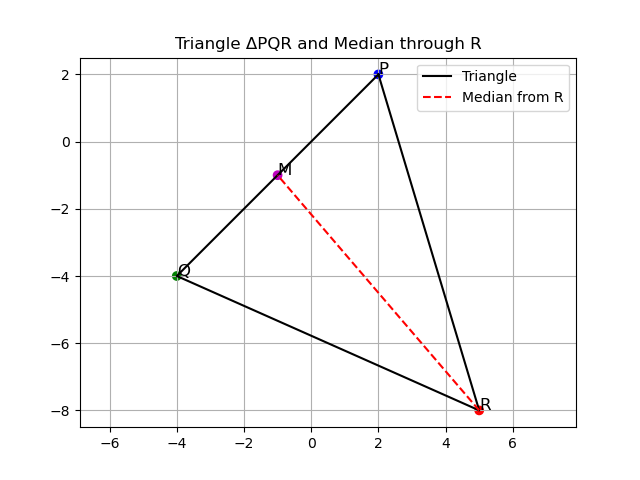
\includegraphics[width=0.5\columnwidth]{../figs/plot.png}
        \caption{Plot of triangle PQR along with median}
        \label{fig:fig}
    \end{figure}
\end{frame}




\end{document}
